\begin{frame}{$d(K^-, n \pi^+ \pi^-)"n"$ event idetification}
  \begin{tabular}{cc}
    \begin{minipage}{0.4\hsize}
      \begin{figure}
        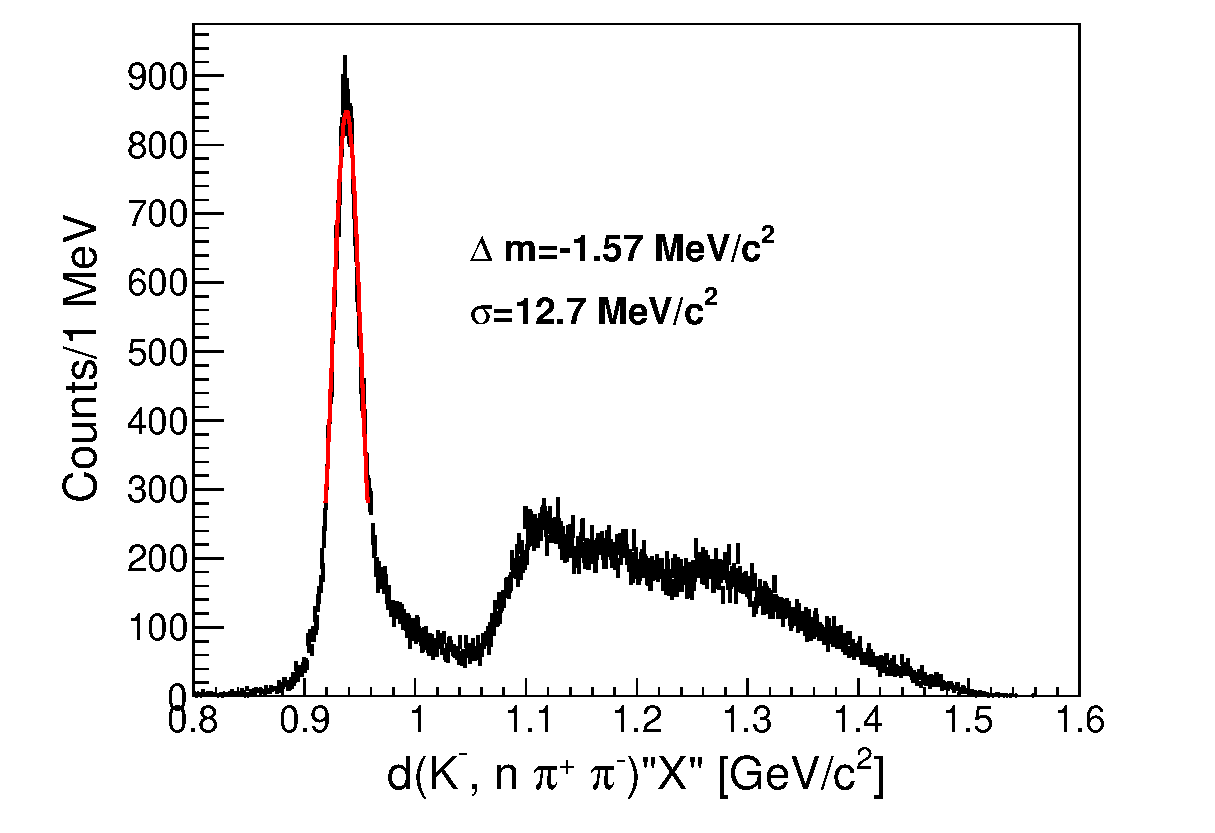
\includegraphics[width=3.5cm]{../pic/Run78/KN_ana_NC170_2sigma/KNpipi_MM_woFit.eps}
      \end{figure}
    \end{minipage}

    \begin{minipage}{0.6\hsize}
      \footnotesize
      Missing neutron was selected by right figure\\
    \end{minipage}
  \end{tabular}
  
  \tminipageThree{
    \begin{figure}
      $K^0$ selection\\
      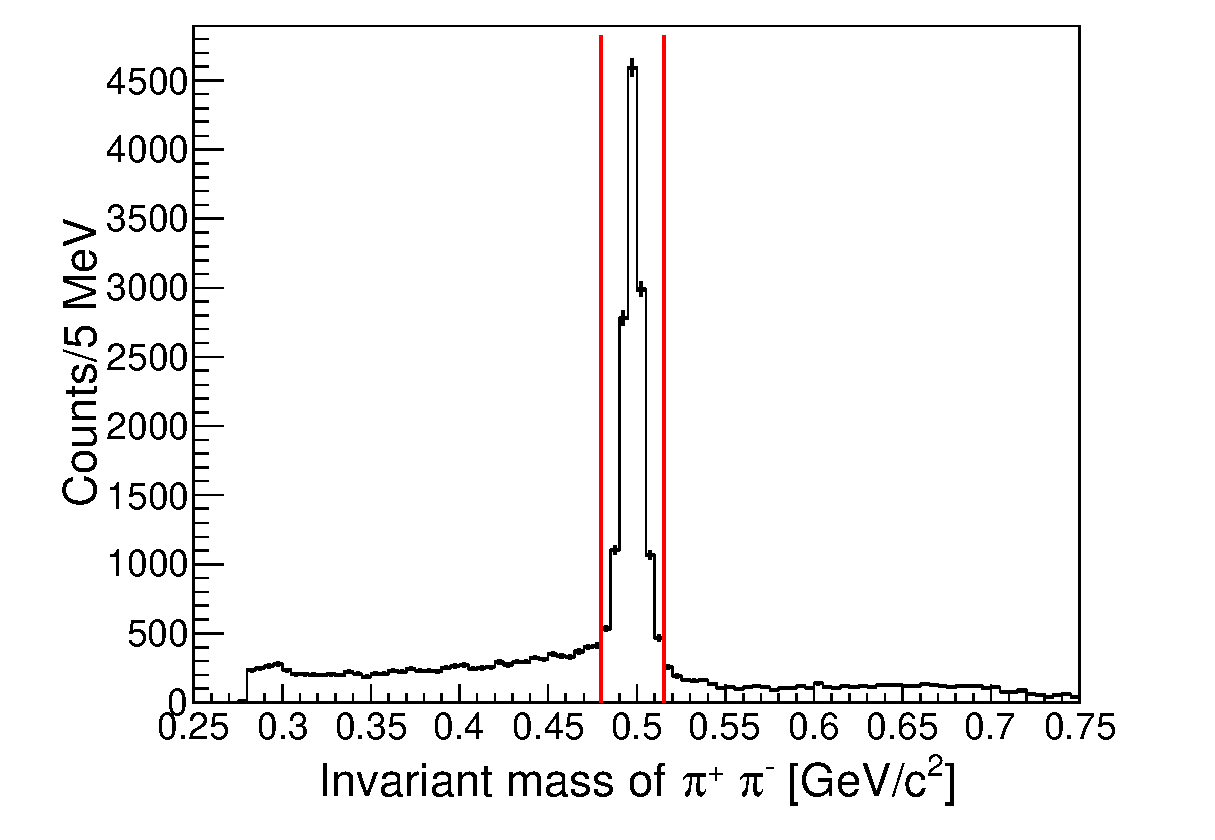
\includegraphics[width=3cm]{../pic/Run78/KN_ana_NC170_2sigma/IM_pipi_woFit.eps}
    \end{figure}
  }{
    \begin{figure}
      $\Sigma^-$ selection\\
      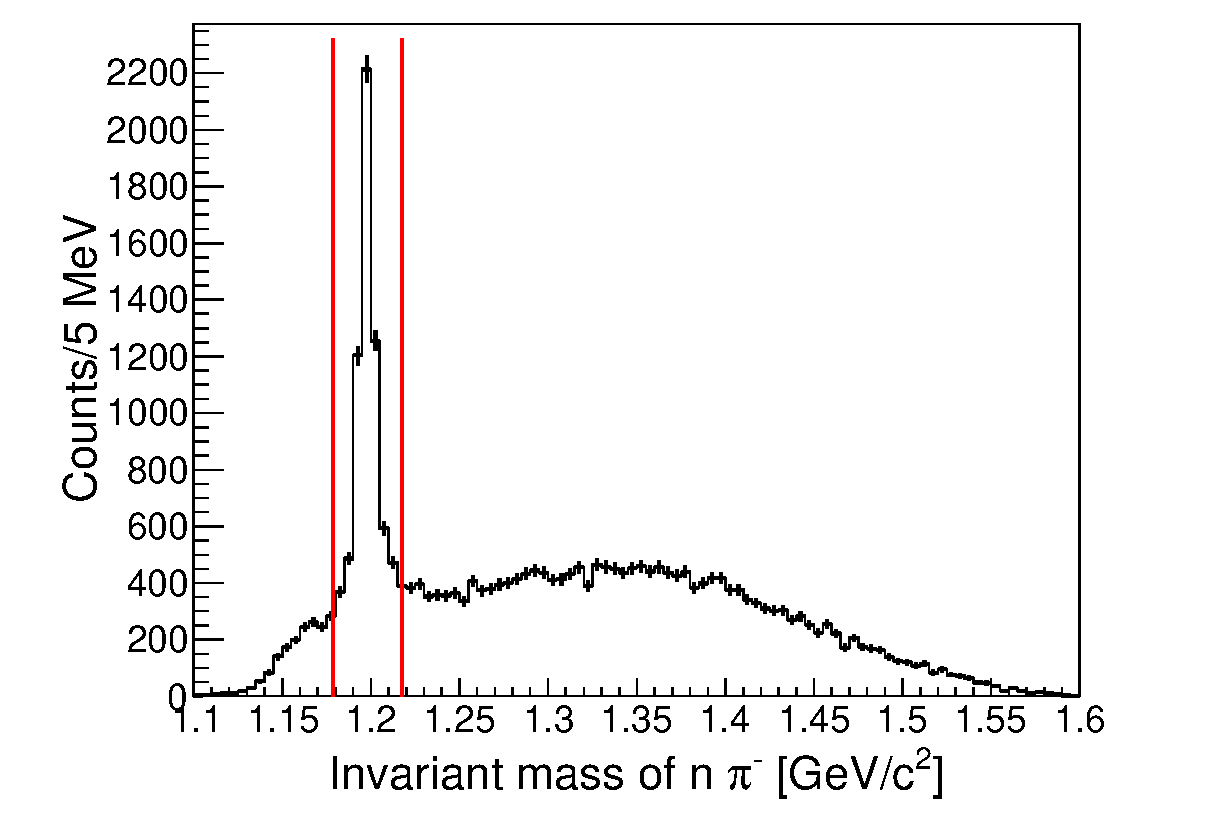
\includegraphics[width=3cm]{../pic/Run78/KN_ana_NC170_2sigma/IM_npim_woFit.eps}

    \end{figure}
  }{
    \begin{figure}
      $\Sigma^+$ selection\\
      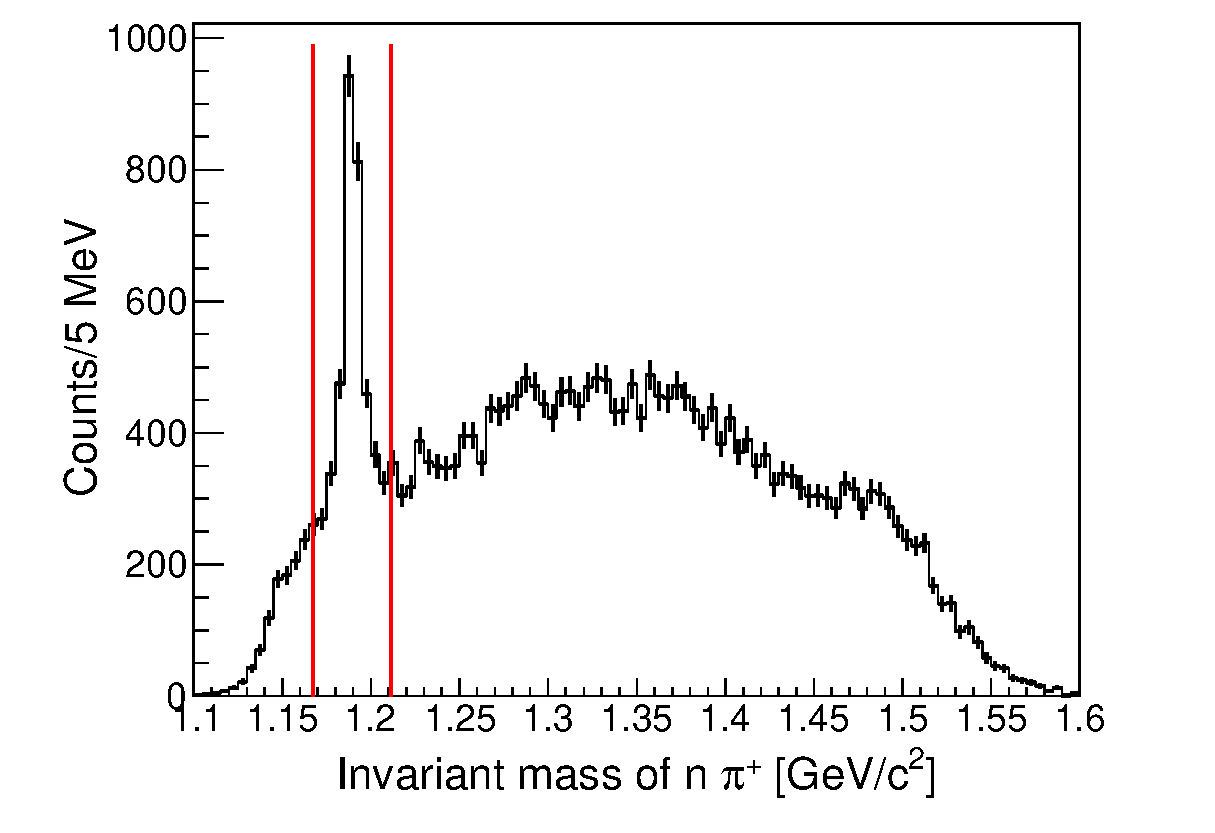
\includegraphics[width=3cm]{../pic/Run78/KN_ana_NC170_2sigma/IM_npip_woFit.eps}
    \end{figure}
  }

  \begin{tabular}{cc}
    \begin{minipage}{0.6\hsize}
      \vspace{-3mm}
      \footnotesize
      These event were identified above figures.
      \begin{enumerate}
      \item $K^- d\rightarrow K^0 n n$\\
        2-step like events was observed.
      \item $K^- d\rightarrow \pi^{\mp}\Sigma^{\pm}$\\
        Forward : Background $\rightarrow$ Negligibly small.\\
        Backward : Main Signal      
      \end{enumerate}

    \end{minipage}
    \begin{minipage}{0.4\hsize}
      \begin{figure}
        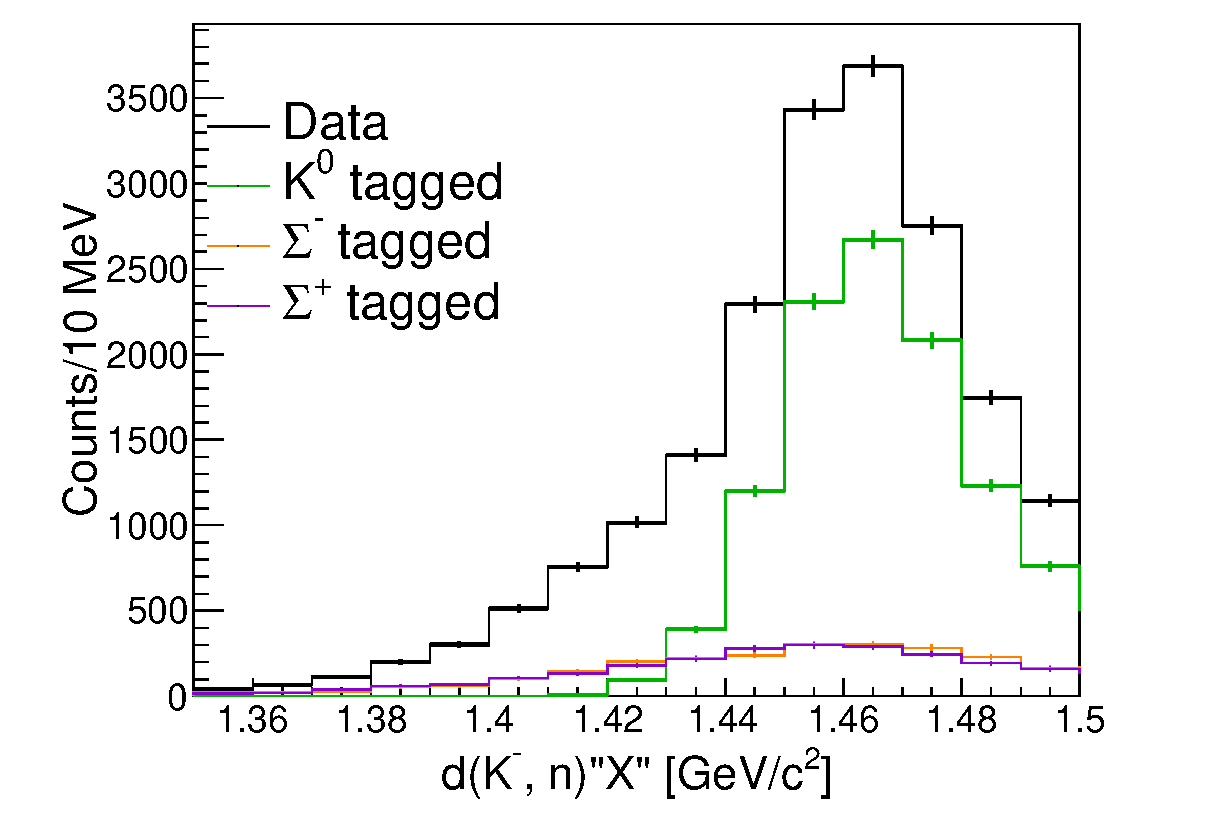
\includegraphics[width=4cm]{../pic/Run78/KN_ana_NC170_2sigma/KN_MM_all.eps}
      \end{figure}
    \end{minipage}
  \end{tabular}
\end{frame}
